\chapter{Descriptive analytics for virtual flow metering systems}

\section{Introduction}
Knowing flow rates from each well is an essential operation of the production systems. It guides operators in production monitoring and decisions making. It assists also in predicting the future performance of the field (Ref). Hence, one of the routine tests of wells is production testing. It is usually conducted as a schedulable test to monitor liquid rates.  Moreover, It is considered as the most popular method of monitoring production and reservoir. Nevertheless, it has several drawbacks. The most frequent restriction is the inadequate resolution to identify trends in liquids rates over short periods of time. Another potential problem is the lack of sufficient testing time to get a representative sample of reservoir fluids.

For each well to be routed to the test separator and tested without having to shut down the entire field, the test separators need a separate flowline. In order to assess the flowrates, stable working conditions must be attained, which might take several hours depending on how far the well is from the separator. Another method of performing a deduction test is to close the well of interest and observe the change. Well testing measures are still commonly employed in production monitoring despite the expense of such approaches. 

Subsequently, another technology called  multiphase Physical flow meters (MPFMs) was developed. This technology found its way in commercialization in the beginning of 1990s.(Falcone et al., 2001). The conceptual idea that stands behind MPFMs is to calculate well multiphase flowrates indirectly by measuring a supplementary properties of the fluid such as, velocities and fraction of phases inside the device (Falcone et al., 2001; Gryzlov, 2011). Several mechanisms were developed to calculate multiphase flow such as, acoustic attenuation, impedance, and gamma densitometers (Falcone et al., 2001).  

This technology has its advantages and disadvantages. One of the important Advantages is the calculation of flow rates without separating the phases. Additionally, these meters are usually installed at the wellhead, due to its low cost and effort of instillation. On the other hand, MPFMs are quite expensive and demand intervention in the event of a failure, which increases the operational cost significantly (Falcone et al., 2001; Patel et al., 2014). Additionally, MPFMs have a certain operating range, beyond which the flowrate predictions' accuracy might dramatically decline. In addition to this, the meters may deteriorate from sand erosion or partial obstruction, which also affects measurement accuracy (Marshall and Thomas, 2015).

Given the previously mentioned difficulties and related expenses, the technology of virtual flow metering (VFM) arises as an attractive technology in oil and gas industry. It depends on either analytical or data driven models for real time calculations of phases production.

The purpose of VFM is to gather Field data that is readily available and utilize it in a model to calculate flowrates (Rasmussen, 2004; Toskey, 2011). This model could be either analytical or data-driven model. Typically, the measurement data consists of: Pump intake pressure and discharge pressure ($P_{intake}$ and $P_{discharge}$). Wellhead pressure and temperature ($WHP$ and $WHT$). Choke opening ($C_{op}$). Pump vibration in X and Y directions ($V_x$ and $V_y$). Variable speed drive current ($I_{VSD}$)

In contrast to production testing and MPFMs, VFM systems do not require installation of an additional hardware, they can, consequently, reduce the capital and operational costs of the field development. At the same time, VFM systems have capabilities to estimate the flowrates in real time and reflect changes of flow conditions accordingly. This is a clear advantage comparing to the well testing approach which assumes constant well flowrates between the tests (Marshall and Thomas, 2015). Moreover, VFM can be used as a standalone solution, or in a combination with a MPFM as a back-up system such that it can use the information from a MPFM to further improve the flowrate estimates.  

In this chapter, VFM classification is introduced based on modeling paradigms. They are classified to first principle and data driven VFMs. In addition, an overview of the concept of both paradigms in VFM systems is presented. Then, a contribution in the area of virtual flow metering on the electrical submersible pumped wells is introduced. Real data from a field is analyzed and handled through multiple machine learning algorithms in order to predict flow rate and water cut. These machine learning algorithms were arranged according to their complexity and ability to be explained. They are multi linear regression, gradient boosted decision trees, and deep learning algorithm (long short-term memory algorithm with convolutional neural network). 

\section{An overview of the concept}
Despite the amount of work done on Virtual Flow Metering and the
diversity of applicable methods and models, there is a lack of an
overview of this. In this paper, we fill this gap and cover the following
objectives:
• Summarize and classify VFM methods, models and computational
procedures.
• Distinguish the differences among the VFM vendors based on publicly available resources.
• Review the reported VFM field experience and the research activity.
• Identify gaps and propose directions for future VFM research and
development.
We believe that this paper will be an asset for readers who want to
get an overview of available VFM solutions, implement the existing
commercial VFM solutions in the field, construct an own VFM or improve the already created one.


The first principles VFM systems are based on mechanistic modeling
of multiphase flows in the near-well region, wells, pipelines and production chokes (Holmås and Løvli, 2011). The models are used together
with the measurements such as pressure and temperature to find accurate estimates of the flowrates. An optimization algorithm adjusts the
flowrates and other tuning parameters to minimize the mismatch between the model predictions and real measurements (Holmås and Løvli,
2011). The production system can be modelled as a whole from the
reservoir to the processing facility, or it can be separated into submodels depending on the available measurement data. First principles
models are currently used in most commercial Virtual Flow Metering
systems.
The data-driven VFM approach is based on collecting the field data
and fitting a mathematical model to it without the exact description of
the physical parameters of the production system such as a wellbore
and choke geometry, flowline wall thickness, etc. This approach is also
referred to as “machine learning” modeling and it has become very
popular in the past several years, not only for oil and gas applications
but for many other applications as well. In this paper, we will call this
approach “data-driven” modeling because in many VFM related publications it was named with this definition. In data-driven modeling, the

fitting process is often called training (Hastie et al., 2009). If the model
is well trained and the exposed conditions are within the range used for
the training, the data-driven model can perform fast and accurate realtime metering. In this approach, deep domain knowledge of production
engineering is not as important as in the first principles models and the
model can be constructed at a lower cost.
In addition to the classification based on the modeling principles,
we may classify approaches based on how time dependency is included
in the model. Based on this, the following sub-classification can be
performed:
• First principles VFM – steady state and dynamic models
• Data-driven VFM – steady state and dynamic models
In the first principles VFM, conservation equations often have a
dynamic form, however, the formulation of the optimization problem is
steady state or quasi-steady state, so that an optimization solver finds
the solution for only one point in time or takes the solution from the last
step as an initial guess for the current time step prediction. In some
cases, even the conservation equations take steady state form or do not
consider time because of its nature, for instance, a choke model
(Perkins, 1993). While it is possible to formulate the VFM optimization
problem in a dynamic way, in the available literature on the first
principles VFM does not consider this approach. The main reason for
this may be the fact that dynamic optimization for first principles VFM
systems is computationally very expensive (Lew and Mauch, 2006). On
the other hand, such methods may have been utilized but not discussed
in the literature.
Apart from dynamic optimization, state estimation techniques such
as Kalman filter approaches can be used in order to create a dynamic
VFM (De Kruif et al., 2008). This approach has been covered in the
research as we will show in the future sections, however, it is not implemented in the commercial software yet. The main reason for this
may be that it requires a high expertise for setting up and using, and it
can be difficult to tune in a robust manner for real field data.
For the large majority of data-driven algorithms used for VFM, the
model formulation is steady state, so that the algorithms consider
pressure and temperature measurements in one point in time to predict
the flowrates at the same time step. At the same time, there are datadriven algorithm structures which have a dynamic formulation, so that
measurements from the past may also be used to estimate the flowrate
at the current time step and some of these algorithms have recently
been studied for VFM applications. In the next sections, we consider
each VFM paradigm in more detail and explain the considerations of
dynamic system behavior by each method based on the used models
and algorithms.


lsa hna hndef 3. First principles VFM systems
3.1. An overview of the concept mn paper 
Timur Bikmukhametov, Johannes Jäschke∗

\section{Exploratory data analysis}
Exploratory data analysis helps to reveal hidden patterns, correlations, and anomalies using various tools such as visualizations (scatter and box plots, histograms, etc.), dimensionality reduction techniques and sometimes unsupervised algorithms. Based on Hair et al. (2013), Our exploratory data analysis includes univariable study that focus on the dependent variables which are flow rate and water cut. Then, a multivariate study that is introduced where we focus on the relationship between dependent and independent variables relationship. Clustering and dimensionality reductions are also studied in this step to investigate the categorical variables. Finally, Basic cleaning is done where we handle the missing data and outliers.

The reported signals are for ESP pumped wells are categorized into 4 different groups. The First group is the well head data that include choke opening ($\%$), wellhead pressure in (psig) , Flow line pressure in (psig), Casing Pressure in (Psig) and wellhead temperature ($^\circ$ F). The second group is the electrical data that include Frequency in Hz, Input Voltage of the three Phases and Variable speed drive (VSD) Output current of the three phases in (Amps). The third group is the operational downhole data that include pump intake pressure in (psia), pump discharge pressure in (psia), Intake Temperature $T_i$ ($^\circ$ C), motor temperature $T_m$ ($^\circ$ C), vibration in 2D ($V_x$, $V_y$) and differential pressure in (psia). The fourth would be MPFM data which are water cut in percent and produced fluid rate in (BPD).

EDA starts with Univariable study in which we just focus on the dependent variable fluid rate and water cut and understand it more. Fig. \ref{fig:density_plot_rate} and Fig \ref{fig:density_plot_watercut} shows the distribution plot for each signal. 

 \begin{figure}
     \centering
     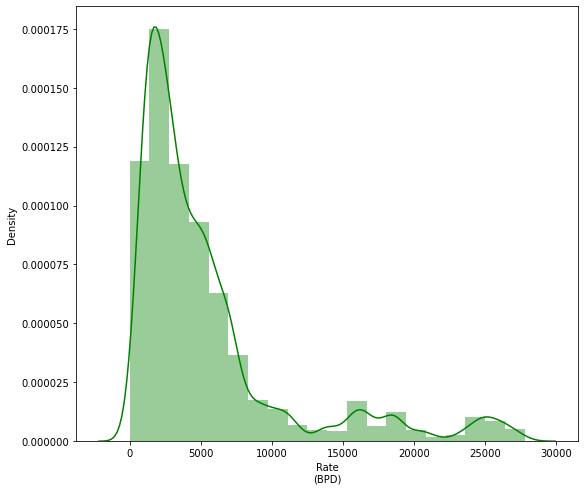
\includegraphics[width = \textwidth]{figures/vfm/desity plot rate.png}
     \caption{Density Plot for fluid rate}
     \label{fig:density_plot_rate}
 \end{figure}

  \begin{figure}
     \centering
     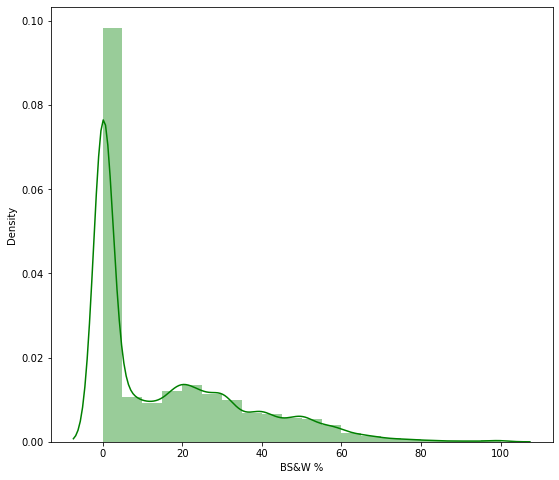
\includegraphics[width = \textwidth]{figures/vfm/desity plot wc.png}
     \caption{Density plot for water cut}
     \label{fig:density_plot_watercut}
 \end{figure}

It is obvious that the rates are skewed left, and some outliers lies above ~15,000 BBLs. The same for water cut above 60 percent. Calculating the skewness and kurtosis for both signals shows that fluid rate has a skewness of 2.09 and kurtosis of 3.98 while the water cut has a skewness of 1.22 and kurtosis of 0.90. It is also shown that a lot of zero production points exist in the data set, which means there are some data points related to non-producing periods. 

Regarding the skewness of fluid rate and water cut, there are two solutions either to get rid of the using kind of outlier removal or to use the log transformation for those target variables, and hence a normal distribution of the independent variable flow rate and water cut that will assist in enhancing modelling results. Regarding the zero reported production points, dropping them is a must as they are just noise data on sensors during the shut-in time. Those will be made in the later step through pre-processing.  

The second step would be a multivariate study in which we study how the dependent variable and independent variables relate. Fig \ref{fig:hist_per_signal}, and \ref{fig:correlation_matrix} show the histogram for each signal as a univariate figure and the correlation matrix for them as a multivariate study for signals. From fig \ref{fig:hist_per_signal}, it is shown that flow rate has an approximately similar distribution with current from the variable speed drive, vibrations in (x, y) and choke opening. Also fig \ref{fig:correlation_matrix} shows that flow rate has a high relation with current from the variable speed drive and choke opening while basic sediments and water are related more to wellhead pressure and a slight inverse proportionality with current and flow rate.     

 \begin{figure}
     \centering
     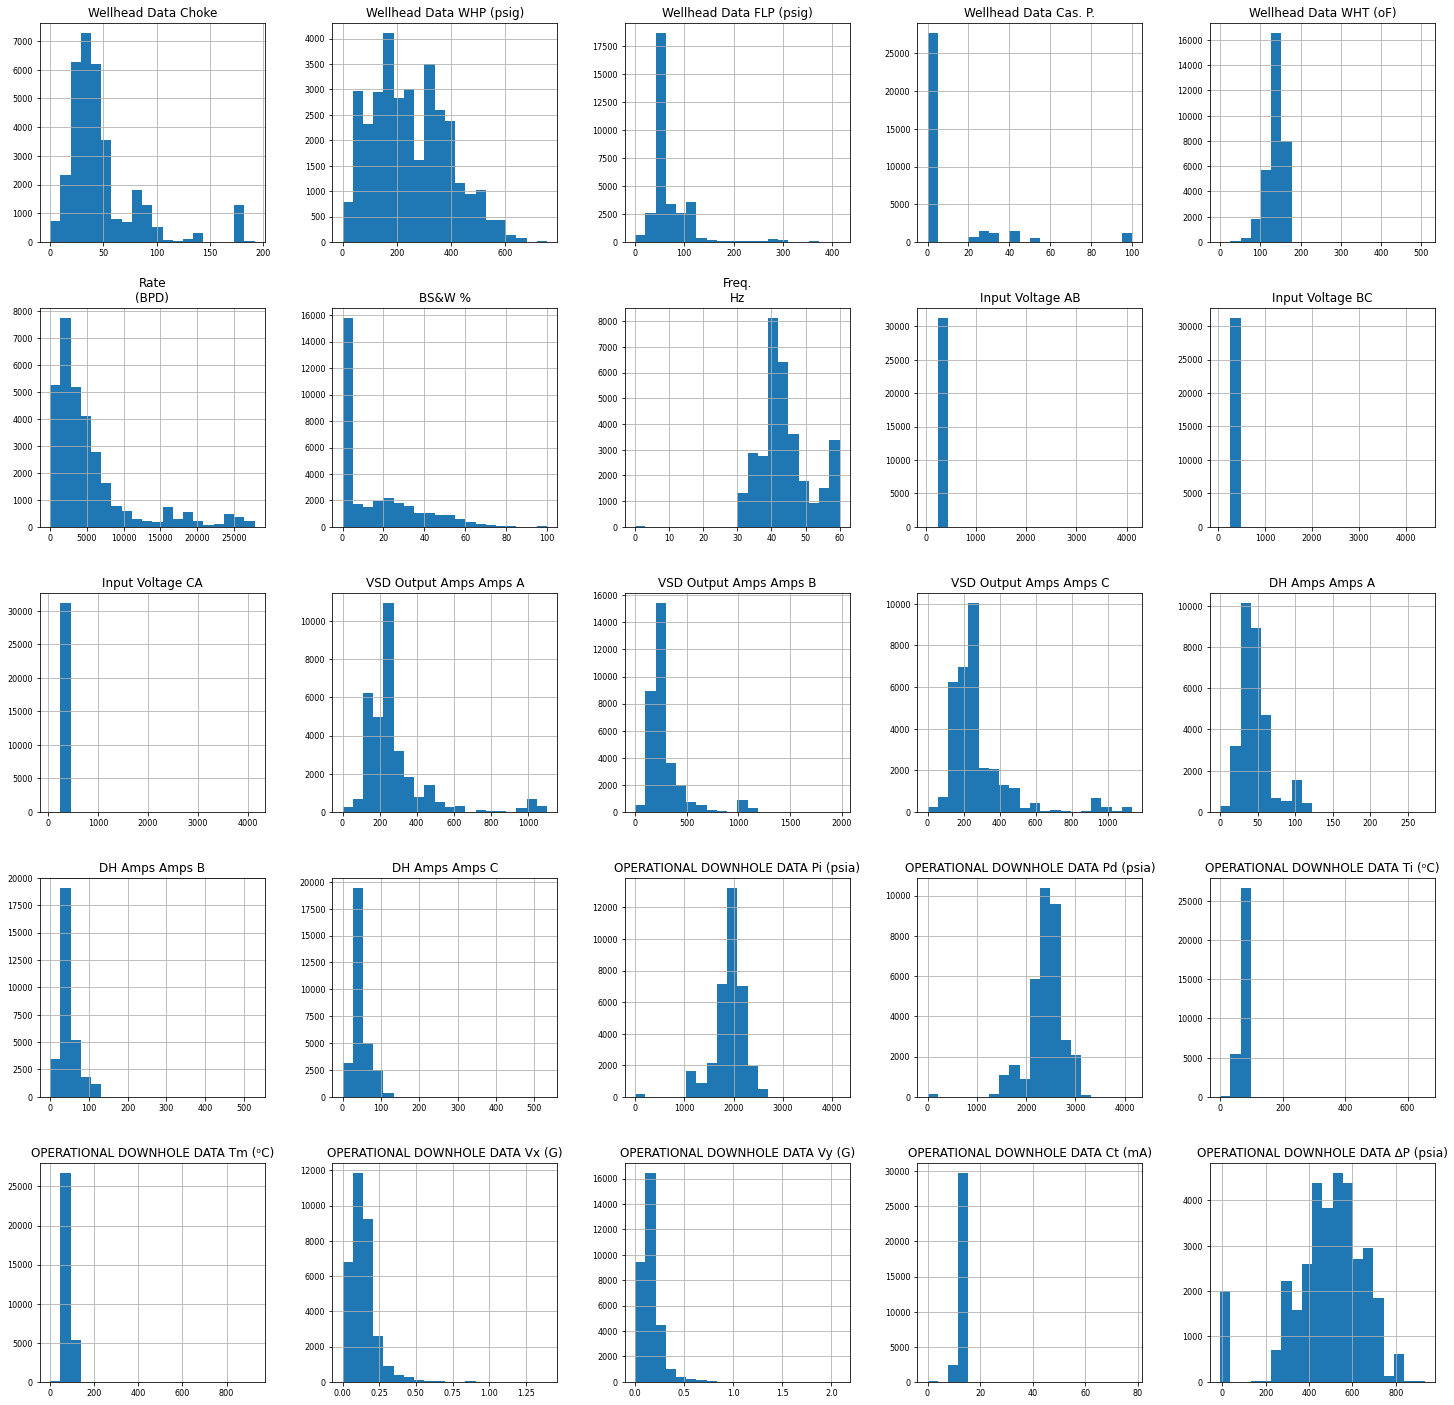
\includegraphics[width = \textwidth]{figures/vfm/pairplot.png}
     \caption{Pair plot histogram for signals}
     \label{fig:hist_per_signal}
 \end{figure}

  \begin{figure}
     \centering
     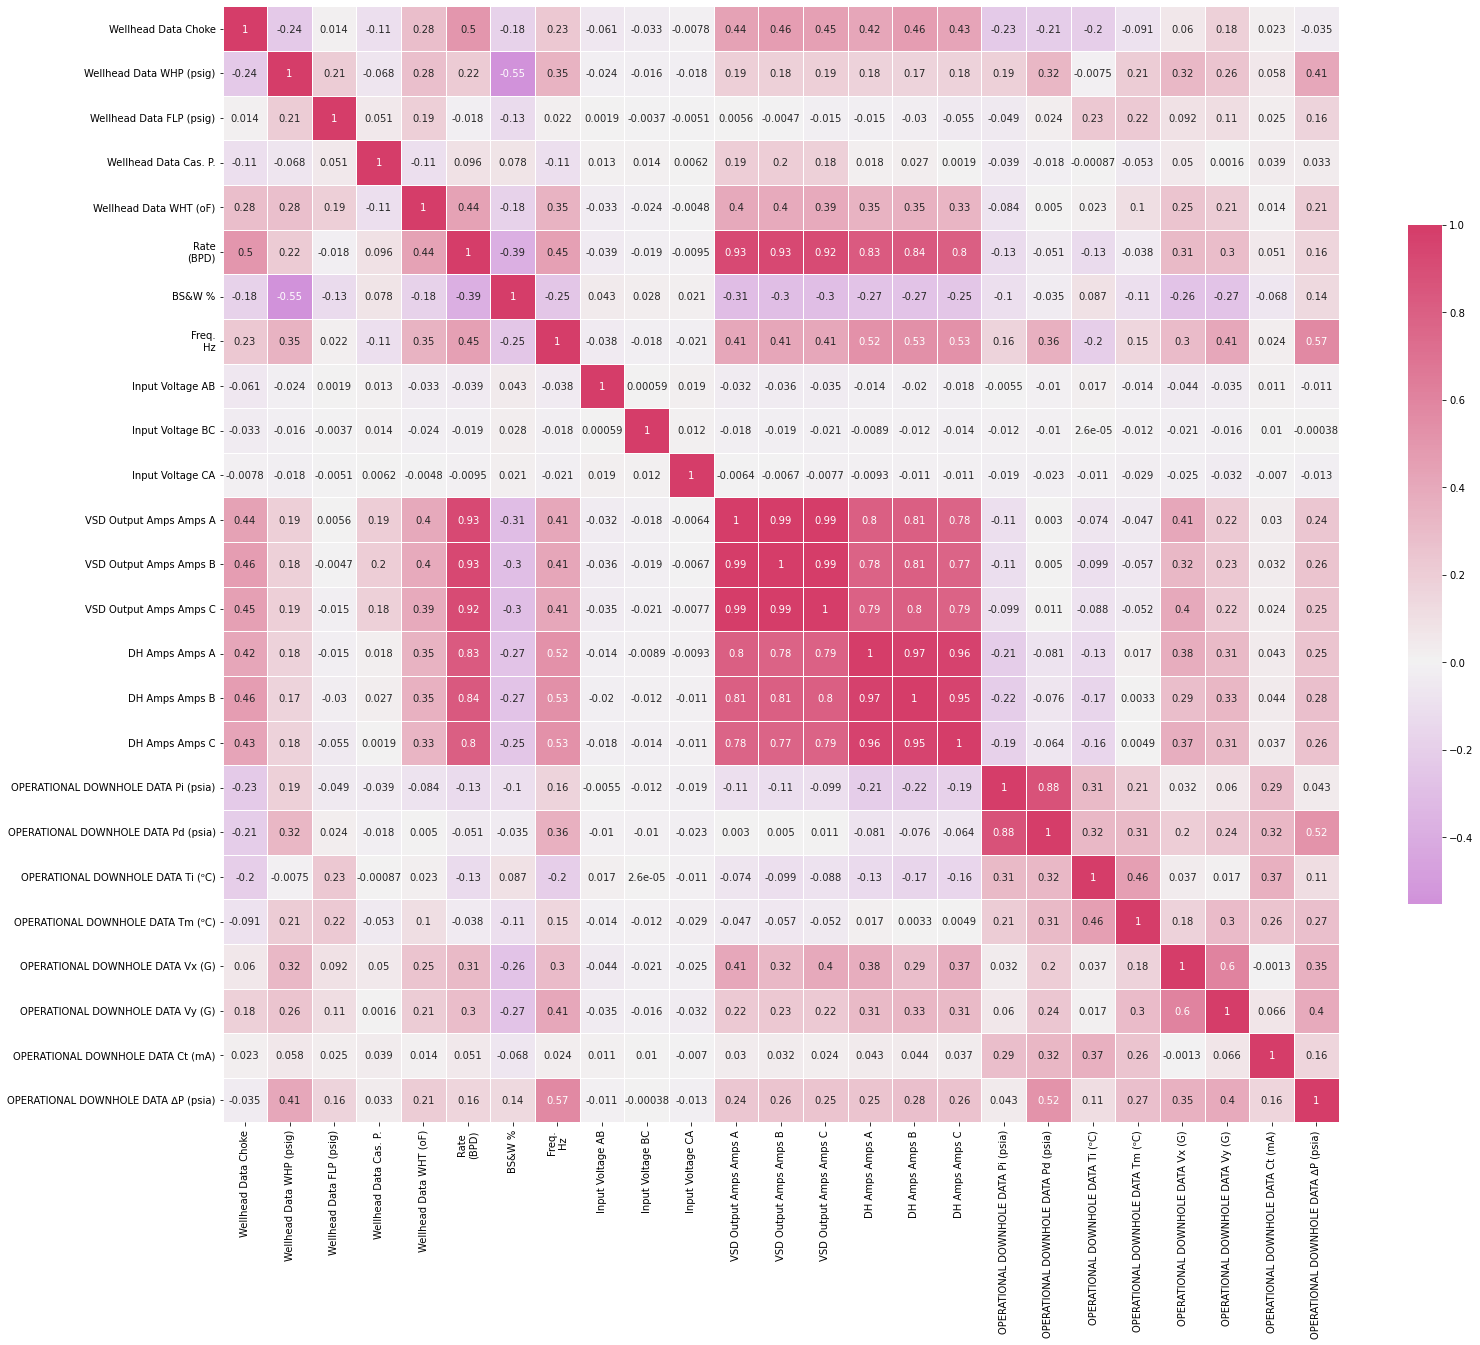
\includegraphics[width = \textwidth]{figures/vfm/correlation plot.png}
     \caption{Correlation matrix for signals}
     \label{fig:correlation_matrix}
 \end{figure}
 
The third study would be on the relationship between flowrate and basic sediments and water with the categorical feature which is a well name. Hence, we explore categorical features with time trends through fig. \ref{fig:trend_oil_rate} and \ref{fig:trend_bsw}. 
Data and demonstrate the locality, spread, and skewness groups of numerical data through fig 7 and 8.

\begin{figure}
     \centering
     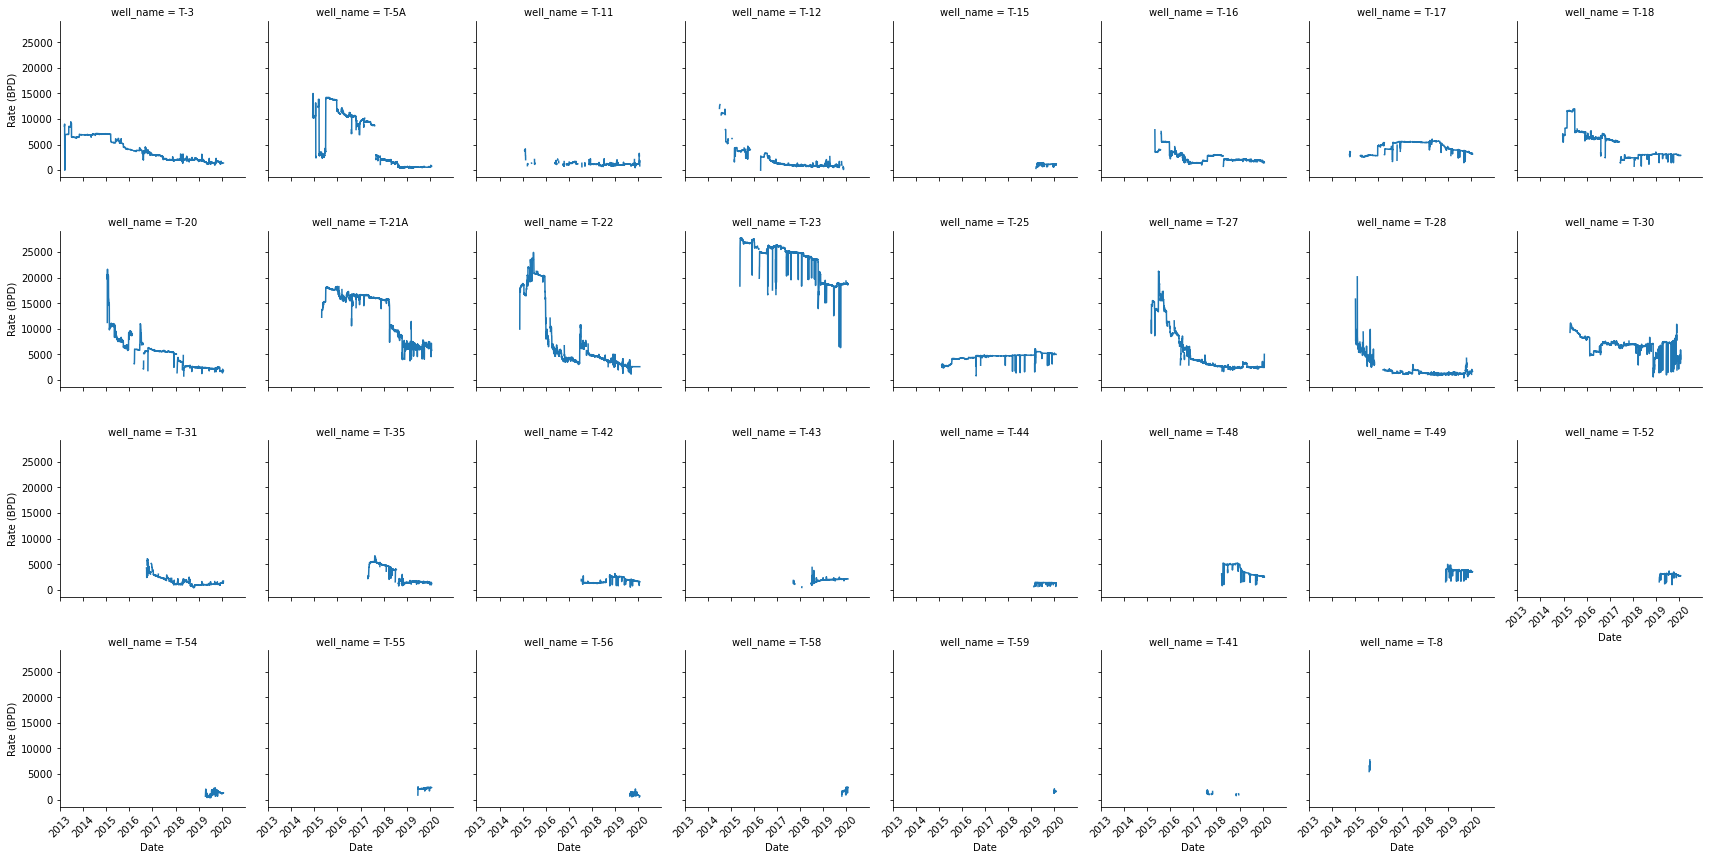
\includegraphics[width = \textwidth]{figures/vfm/trend oil rate.png}
     \caption{Time plot of flow rate for each well}
     \label{fig:trend_oil_rate}
\end{figure}  

\begin{figure}
     \centering
     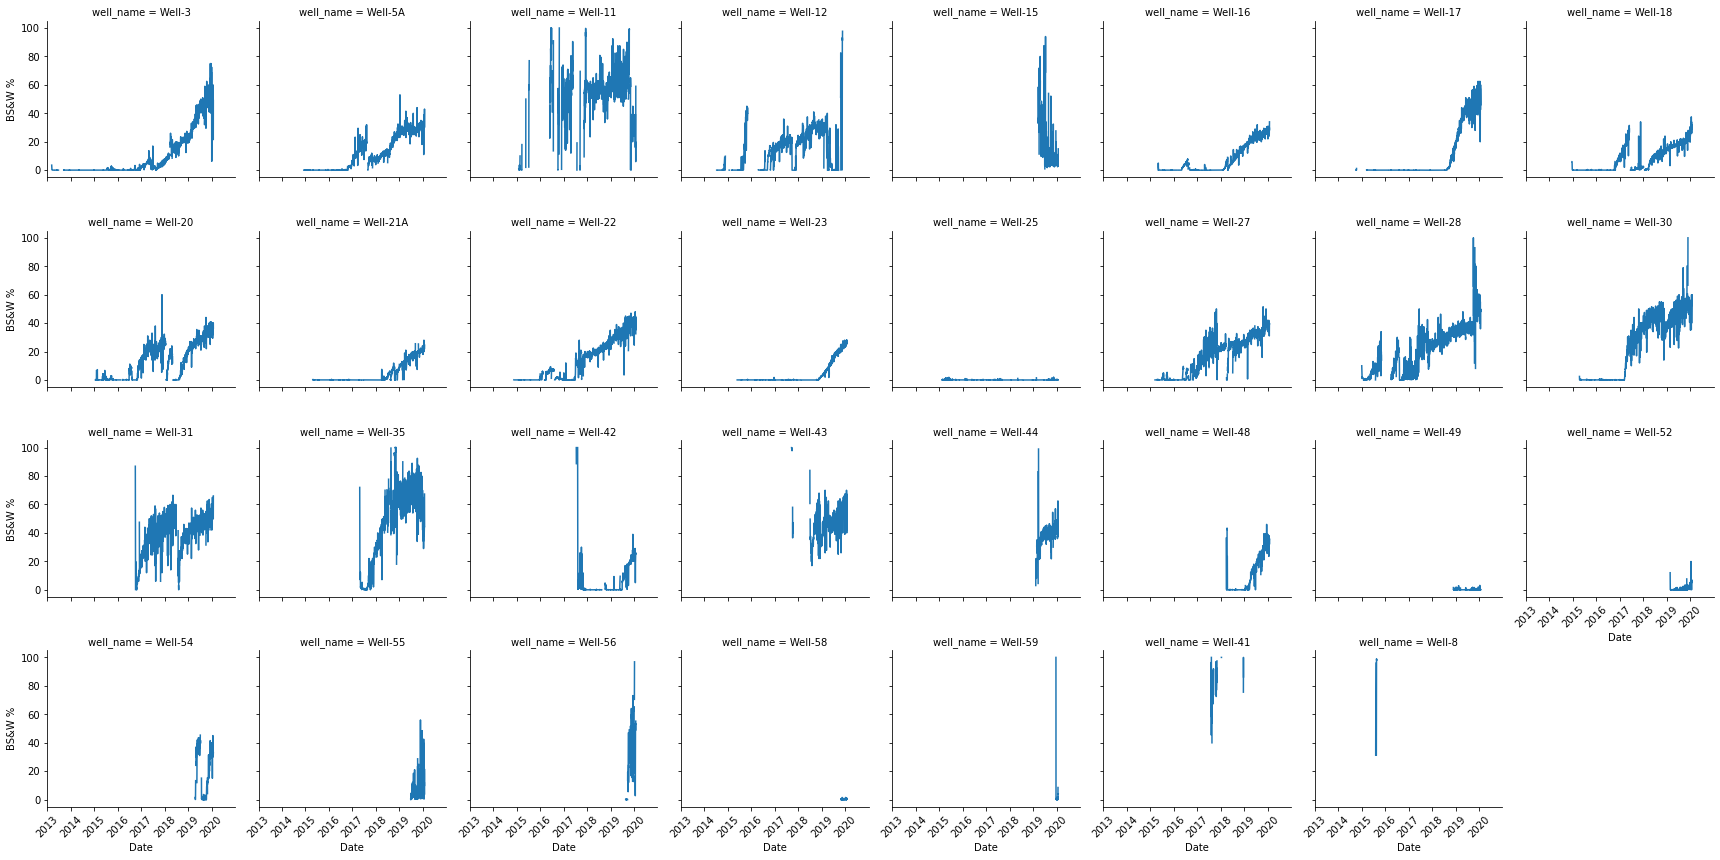
\includegraphics[width = \textwidth]{figures/vfm/trend bsw.png}
     \caption{Time plot for Basic sediments and water for each well}
     \label{fig:trend_bsw}
\end{figure}

\begin{figure}
     \centering
     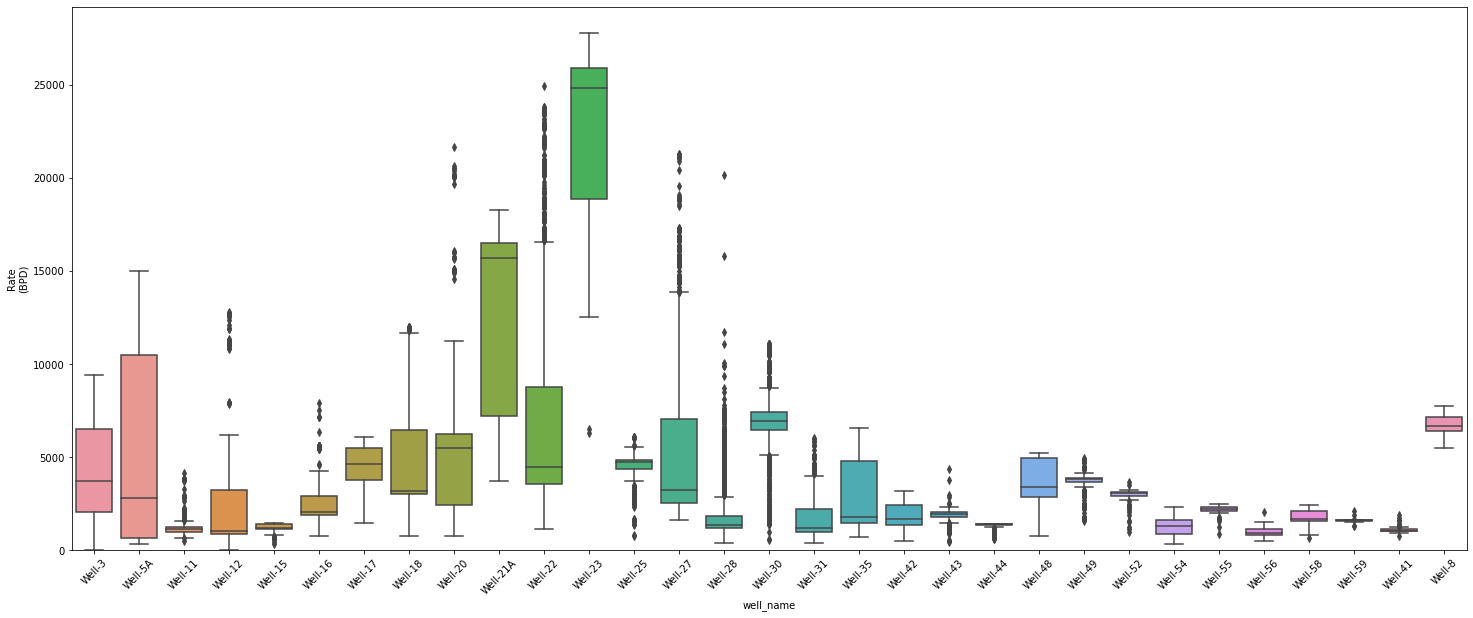
\includegraphics[width = \textwidth]{figures/vfm/box plot rate.png}
     \caption{Boxplot of flow rate for each well}
     \label{fig:correlation_matrix}
\end{figure}

\begin{figure}
     \centering
     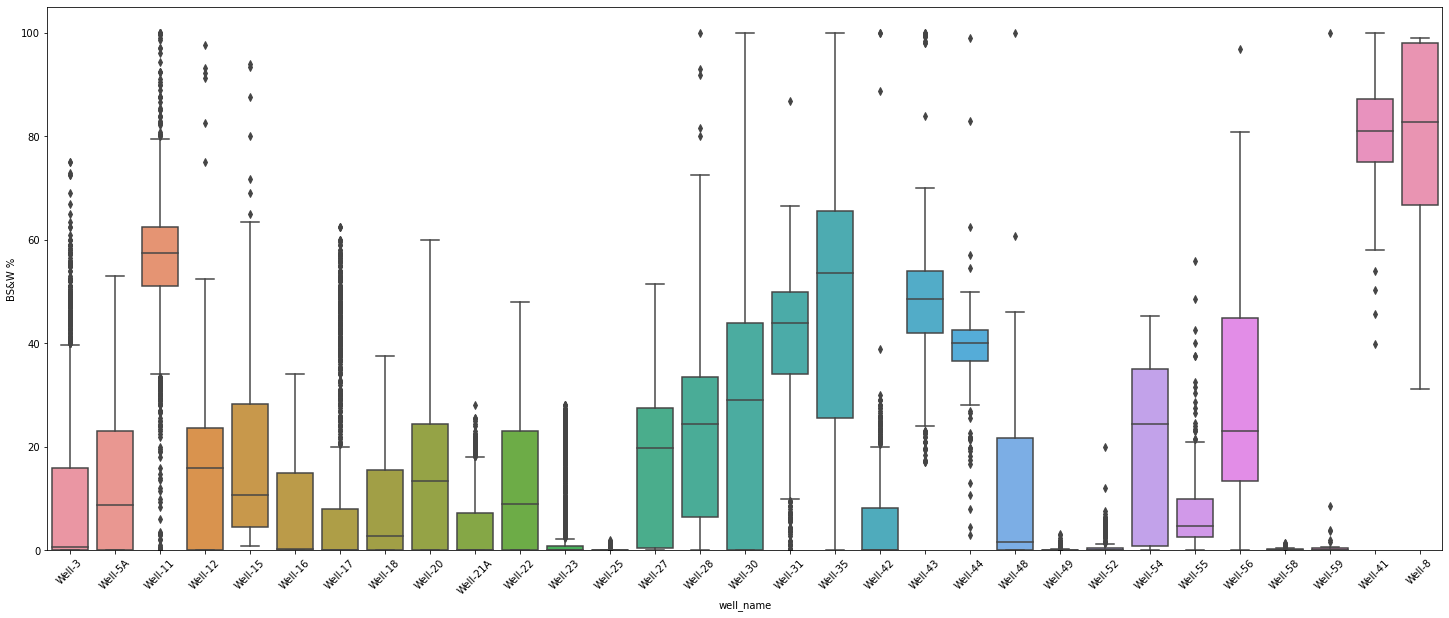
\includegraphics[width = \textwidth]{figures/vfm/box plot bsw.png}
     \caption{box plot of basic sediments and water for each well}
     \label{fig:correlation_matrix}
\end{figure}

The missing data points are dropped for the main five main signals. Those are production data because it does not make sense to have zero production reported sensor measurements. The other three signals are variable speed drive output current, pump intake pressure, Frequency, and discharge pressure. Then, the missing data for all signals are presented in table \ref{tab:missing_data}. Hence, The 3 phase input voltage signals (AB, CA, and BC) are dropped because, in addition to their small correlation factor with fluid rate and basics sediments and water signals that are shown in fig \ref{fig:correlation_matrix}, they also have the highest missing values that are shown in table \ref{tab:missing_data}.  Then, the motor current signal is removed because it is highly correlated with variable speed drive output recorded current and has been considered one of the highest missing signals.

\begin{table}[]
\resizebox{\textwidth}{!}{%
\begin{tabular}{|l|l|S[round-mode = places]|}
\hline
Reported Signal             & Total & Percent  \\ \hline
Input Voltage AB            & 2098  & 0,066624 \\ \hline
Input Voltage CA            & 2098  & 0,066624 \\ \hline
Input Voltage BC            & 2098  & 0,066624 \\ \hline
DH Amps A                   & 1469  & 0,04665  \\ \hline
DH Amps C                   & 1468  & 0,046618 \\ \hline
DH Amps B                   & 1468  & 0,046618 \\ \hline
T_m ($^\circ$C)                     & 1446  & 0,045919 \\ \hline
C_t (mA)                     & 1444  & 0,045856 \\ \hline
V_x (G)                      & 1443  & 0,045824 \\ \hline
T_i (ᵒC)                     & 1440  & 0,045729 \\ \hline
V_y (G)                      & 1440  & 0,045729 \\ \hline
BS\&W (\%)                    & 590   & 0,018736 \\ \hline
Wellhead Data FLP (psig)    & 341   & 0,010829 \\ \hline
Wellhead Data WHT (oF)      & 280   & 0,008892 \\ \hline
Wellhead Data Cas. P.       & 12    & 0,000381 \\ \hline
P_d (psia)                   & 0     & 0        \\ \hline
Wellhead Data Choke opening & 0     & 0        \\ \hline
VSD Output Amps Amps A      & 0     & 0        \\ \hline
P_i (psia)                   & 0     & 0        \\ \hline
VSD Output Amps C           & 0     & 0        \\ \hline
VSD Output Amps B           & 0     & 0        \\ \hline
Wellhead Data WHP (psig)    & 0     & 0        \\ \hline
Frequency (Hz)              & 0     & 0        \\ \hline
Rate (BPD)                  & 0     & 0        \\ \hline
∆P (psia)                   & 0     & 0        \\ \hline
\end{tabular}%
}
\caption{Missing Data Per Signal}
\label{tab:missing_data}
\end{table}

Regarding data transformation, figure \ref{fig:prob_dist_rate} shows that the target flow rate probability density distribution has skewness from the normal distribution. Hence, the log transformation is used on flow rate sensor measurements. The log transformation is a widely used method to address skewed data. In other words, to make the data as normal as possible and thus increase the validity of the associated statistical modelling, log transformation data is used instead of the Cartesian transformation. Figure \ref{fig:prob_dist_rate} shows the probability plot and the distribution for flow rate before and after log transformation.  

\begin{figure}
     \centering
     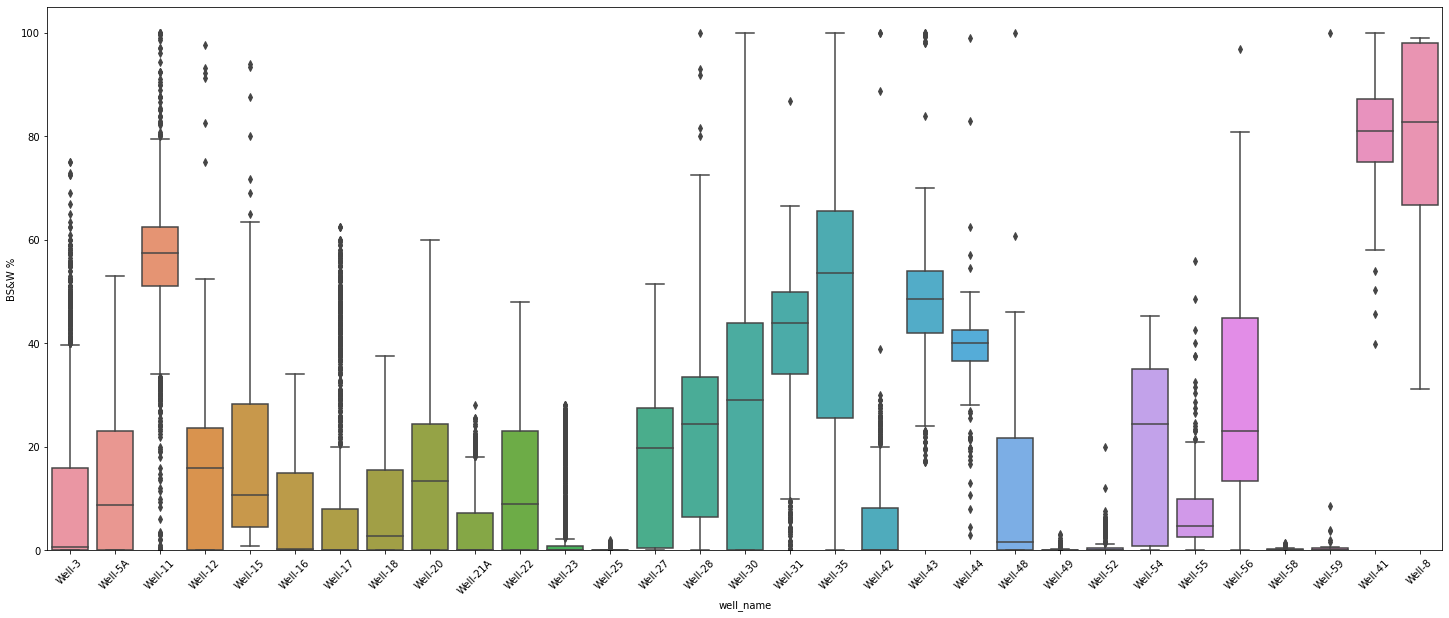
\includegraphics[width = \textwidth]{figures/vfm/box plot bsw.png}
     \caption{the probability plot and the distribution for flow rate}
     \label{fig:prob_dist_rate}
\end{figure}

Another important study in data exploration is the usage of unsupervised learning techniques to unleash any grouping in the input data. Hence, principal component analysis and -Kmean algorithms are studied. Figs \ref{fig:pca_well} and \ref{fig:pca_freq} show the projection of the input signals on the first two principal components. There is a slight clustering per well and a slight grading of the input signals with pump frequency, which means we may have a slight enhancement in modelling either by using well name or frequency as a categorical parameter. Also, K-means has been applied to the input signals to study the effect of grouping the data before modelling. Fig.   \ref{fig:sil1_6} shows the silhouette analysis of k means clustering.  Silhouette analysis can be used to study the separation distance between the resulting clusters. The silhouette plot displays a measure of how close each point in one cluster is to points in the neighbouring clusters and thus provides a way to assess parameters like the number of clusters visually. This measure has a range of [-1, 1]. Silhouette coefficients near +1 indicate that the sample is far away from the neighbouring clusters. A value of 0 indicates that the sample is very close to the decision boundary between two neighbouring clusters and negative values indicate that those samples might have been assigned to the wrong cluster.  

From \ref{fig:sil1_6} for n_clusters = 2 The average silhouette_score is : 0.251, for n_clusters = 3 The average silhouette_score is : 0.2667, for n_clusters = 4 The average silhouette_score is : 0.259, for n_clusters = 5 The average silhouette_score is : 0.282 
the highest score was with 5 clusters and it is still very small .282. Therefore, clustering is not recommended in that case. 
 

\begin{figure}
     \centering
     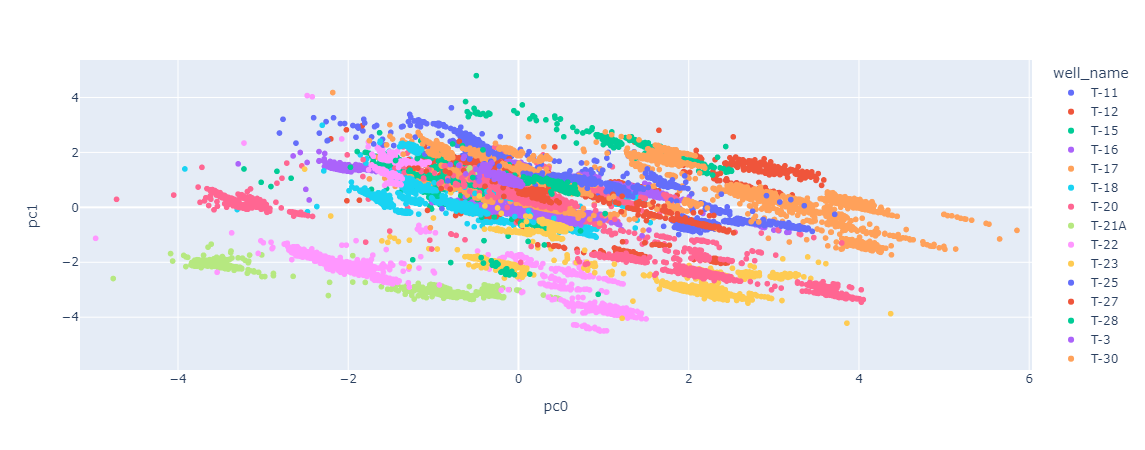
\includegraphics[width = \textwidth]{figures/vfm/pca_well.png}
     \caption{PCA of the input signals per well}
     \label{fig:pca_well}
\end{figure}
 
\begin{figure}
     \centering
     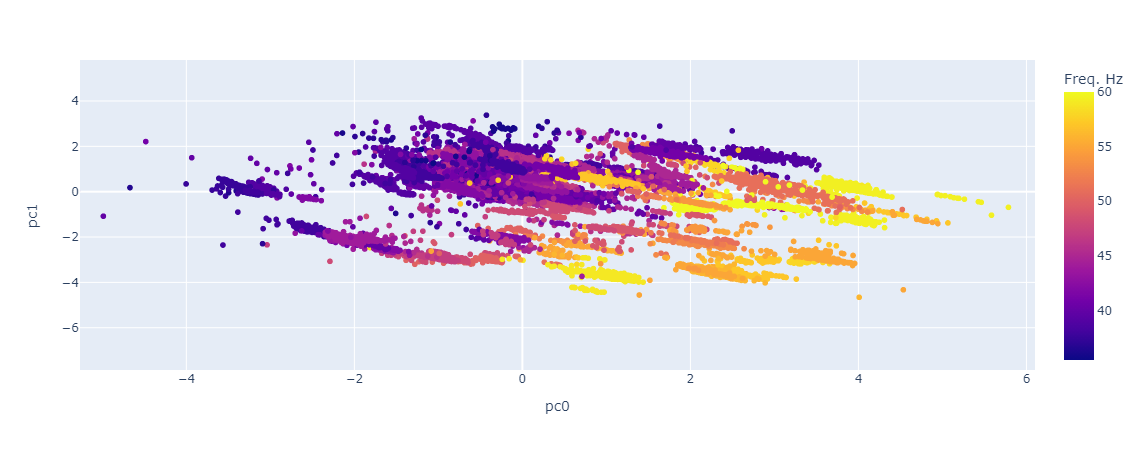
\includegraphics[width = \textwidth]{figures/vfm/pca_freq.png}
     \caption{PCA of the input signals With Frequency}
     \label{fig:pca_freq}
\end{figure}

\begin{figure}    
    \begin{subfigure}{\textwidth}
      \centering
         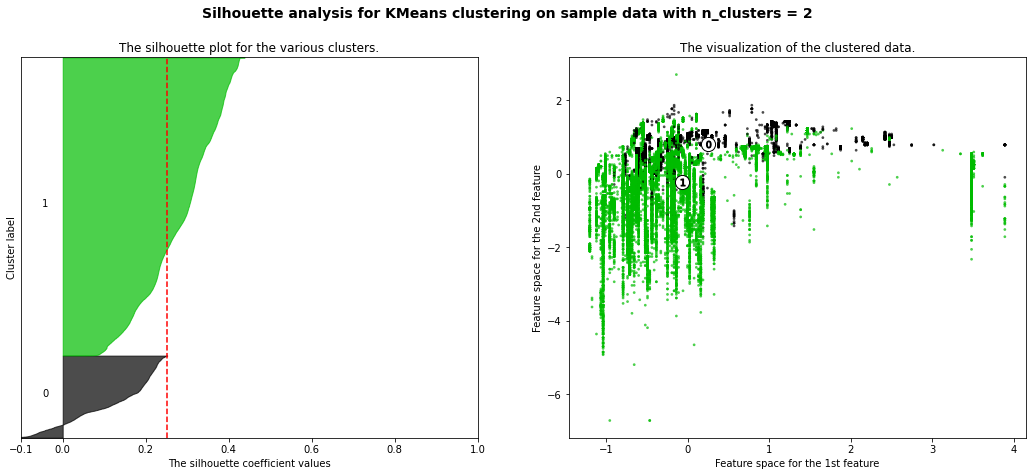
\includegraphics[width = .8\textwidth]{figures/vfm/sil1.png}
         \caption{Silhouette Analysis for 2 clusters}
         \label{fig:sil}
    \end{subfigure}%

    \begin{subfigure}{\textwidth}
      \centering
      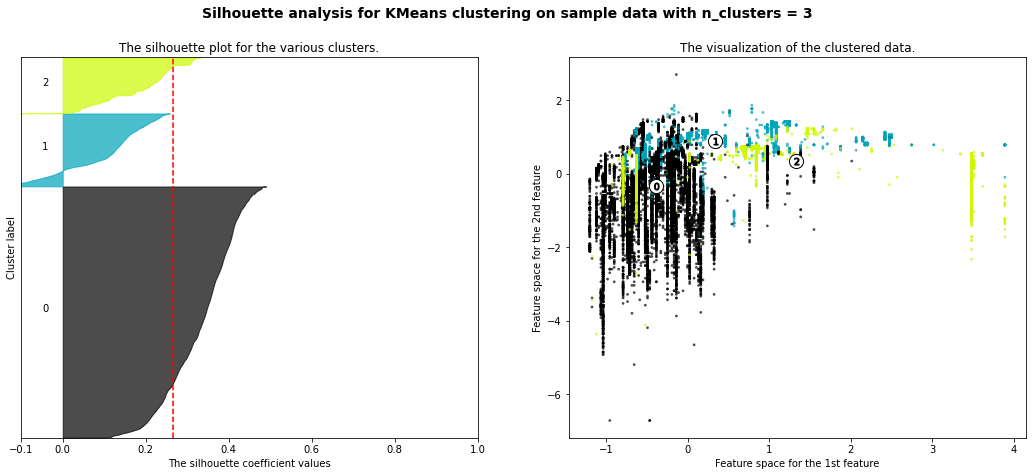
\includegraphics[width=.8\linewidth]{figures/vfm/sil2.png}
      \caption{Silhouette Analysis for 3 clusters}
      \label{fig:sfig2}
    \end{subfigure}

    \begin{subfigure}{\textwidth}
      \centering
      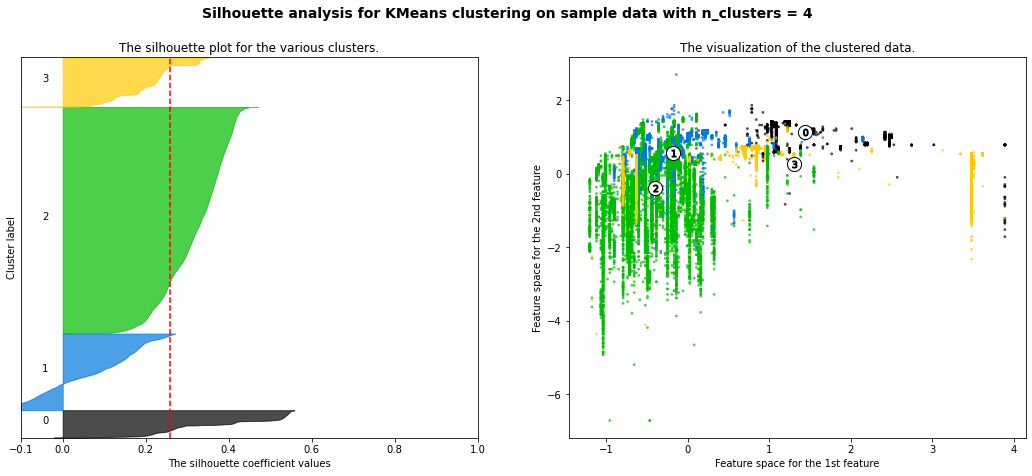
\includegraphics[width=.8\linewidth]{figures/vfm/sil3.png}
      \caption{Silhouette Analysis for 4 clusters}
      \label{fig:sfig2}
    \end{subfigure}
\end{figure}  

\begin{figure}
  \ContinuedFloat 
    \begin{subfigure}{\textwidth}
      \centering
      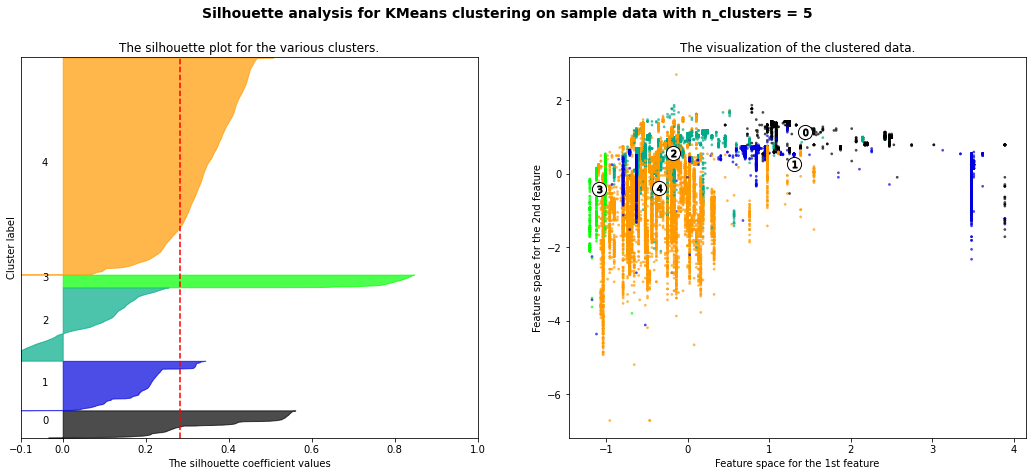
\includegraphics[width=.8\linewidth]{figures/vfm/sil4.png}
      \caption{Silhouette Analysis for 5 clusters}
      \label{fig:sfig2}
    \end{subfigure}

    \begin{subfigure}{\textwidth}
      \centering
      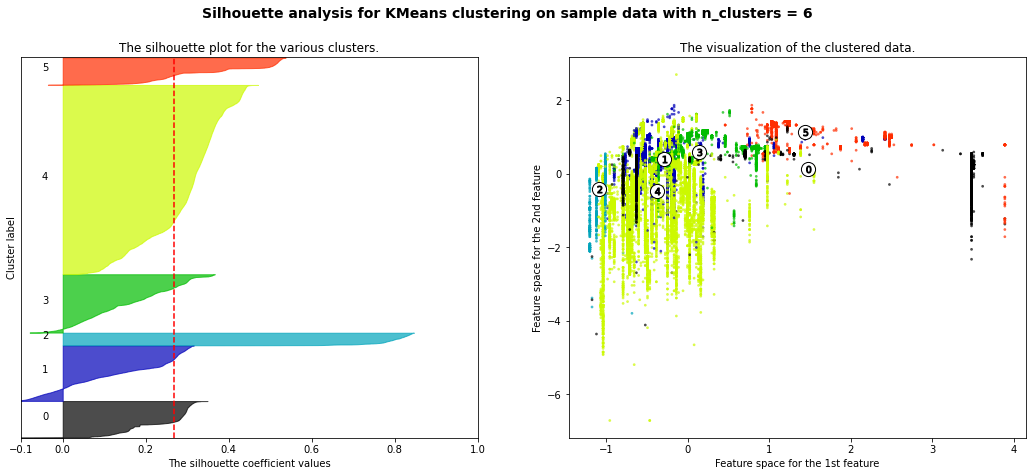
\includegraphics[width=.8\linewidth]{figures/vfm/sil5.png}
      \caption{Silhouette Analysis for 6 clusters}
      \label{fig:sfig2}
    \end{subfigure}
\caption{Silhouette Analysis from 2 to 6 clusters}
\label{fig:sil1_6}
\end{figure}


\section{Feature permutation}
A custom type of feature permutation importance model has been applied. feature permutation importance is a model-agnostic method that provides insights into a machine learning model’s behavior. It estimates and ranks feature importance based on the impact each feature has on the trained machine learning model’s predictions.

Feature permutation measures the predictive value of a feature for our estimator. It evaluates a specific input by evaluating how the average prediction error for all models in which this input incorporated. 

The following summarizes the main steps in computing our custom feature permutation importance:
1-	Split the dataset into train and test sets
2-	Get all permutations for the input features.
3-	Randomly shuffle the feature column in the given dataset.
4-	Train each model on the same training set
5-	Calculate the prediction error on the test dataset. 
6-	Store the used input features with the training and testing results.
7-	Repeat the preceding three steps multiple times and save the results in experiments dataframe
8-	For each input feature, the Average error reported for all models it has contributed on. Averaging mitigates the effects of random shuffling.
9-	Rank the features based on the average impact each feature has on the model’s score. Features that have contributed to smallest error models are assigned with higher importance. 
Based on the feature rotation random search, Table 3 and 4 shows the signals recommended as input for flow rate and water cut respectively. Detailed results of this study is reported in Appendix A

\begin{table}[]
\resizebox{\columnwidth}{!}{%
\begin{tabular}{|l|l|}
\hline
Signal                                & Average MAE \\ \hline
VSD Output Amps   Amps A              & 0,039       \\ \hline
OPERATIONAL   DOWNHOLE DATA Pd (psia) & 0,040       \\ \hline
OPERATIONAL DOWNHOLE DATA Pi (psia)   & 0,041       \\ \hline
Freq. Hz                              & 0,041       \\ \hline
Wellhead Data   Choke                 & 0,041       \\ \hline
Wellhead Data WHP   (psig)            & 0,041       \\ \hline
Wellhead Data FLP   (psig)            & 0,041       \\ \hline
OPERATIONAL   DOWNHOLE DATA Tm (ᵒC)   & 0,041       \\ \hline
Wellhead Data   Cas. P.               & 0,041       \\ \hline
OPERATIONAL   DOWNHOLE DATA ∆P (psia) & 0,041       \\ \hline
Wellhead Data WHT   (oF)              & 0,041       \\ \hline
OPERATIONAL   DOWNHOLE DATA Ti (ᵒC)   & 0,041       \\ \hline
OPERATIONAL   DOWNHOLE DATA Vy (G)    & 0,042       \\ \hline
\end{tabular}%
}
\caption{Feature Rotation for flowrate}
\label{tab:rate_rotation}
\end{table}


\begin{table}[]
\resizebox{\columnwidth}{!}{%
\begin{tabular}{|l|l|}
\hline
Signal                                & Average MAE \\ \hline
VSD Output Amps A              & 2,16        \\ \hline
OPERATIONAL   DOWNHOLE DATA $\Delta$P (psia) & 2,20        \\ \hline
Wellhead Data WHP   (psig)            & 2,21        \\ \hline
OPERATIONAL   DOWNHOLE DATA P_d (psia) & 2,21        \\ \hline
Wellhead Data   Choke                 & 2,22        \\ \hline
OPERATIONAL DOWNHOLE DATA P_i (psia)   & 2,24        \\ \hline
OPERATIONAL   DOWNHOLE DATA T_m ($^\circ$ C)   & 2,31        \\ \hline
OPERATIONAL   DOWNHOLE DATA V_y (G)    & 2,31        \\ \hline
OPERATIONAL   DOWNHOLE DATA T_i ($^\circ$ C)   & 2,35        \\ \hline
Wellhead Data   Cas. P.               & 2,38        \\ \hline
Wellhead Data FLP   (psig)            & 3,40        \\ \hline
Freq. Hz                              & 3,41        \\ \hline
Wellhead Data WHT ($^\circ$ F)              & 4,41        \\ \hline
\end{tabular}%
}
\caption{Feature Rotation for BS\&W}
\label{tab:wc_rotation}
\end{table}



\section{ALGORITHMS}
Usually, the ML models perform differently based on the given data. That is why there is no golden rule for picking the specific model for a certain task. The best model can be only chosen after the data is analyzed and the different ML models are compared. In this section, we describe the algorithms that have been used in this research. These algorithms start with symbolic regression, support vector regressor (SVR) and from deep learning algorithms, 1D \ac{CNN} are used to predict flow rates and BS\&W. 

\subsection{Symbolic regression}

For discovering hidden relationships between variables in Symbolic Regression is accomplished by turning data into explicit mathematical formulas.
The steps of a Symbolic Regression optimization are:
	Take a dataset with two or more columns;
	Propose formulas for one of the columns as a function of the other ones;
	Evaluate the errors and keep track of the record-holders.

Intrinsic stochasticity is involved: random formulas must be sequentially tried. Since too many possible formulas exist, a clever algorithm must be used.
It is a powerful tool to help understand the underlying dynamics of some observed phenomenon.
Instead of fitting numbers to some presumed model, as your classic regression does, this method optimizes the functional form itself of the relationship between the variables.
This can often help you discover nonlinear correlations between your variables that regular regression models could just not predict.

However, care must be taken to avoid over-fit models, where spurious correlations between the variables are given too much merit leading to good fits with little predictive value. To avoid this risk, the use of cross-validation is recommended.
The power of symbolic regression comes from the fact that all you need is known: your data. The method takes care of turning its intrinsic distributions and correlations into meaningful models.

\subsection{Deep Learning (\ac{LSTM}  and Conv1D)}  
For massive data and high computational performance, deep learning models have recently shown great advantages in automatically extracting and learning multivariate data features. In particular, the Recurrent Neural Network (RNN) and its various improved models have been applied to feature extraction of time series data. In this study, we propose a general framework for multivariate prediction problems, including \ac{CNN} and Bi-\ac{LSTM}. CNN is used to extract the horizontal relationship of multidimensional variables before the Bi-LSTM network layer, while Bi-LSTM is used to learn the timing relationships of features obtained by CNN and predict based on this.

Our model consists of two main parts. CNN is used to extract the lateral features of multidimensional data, and Bi-LSTM is used to extract the temporal features of the data which is shown in Fig. \ref{fig:lstm_cnn}.

\begin{figure}
    \centering
    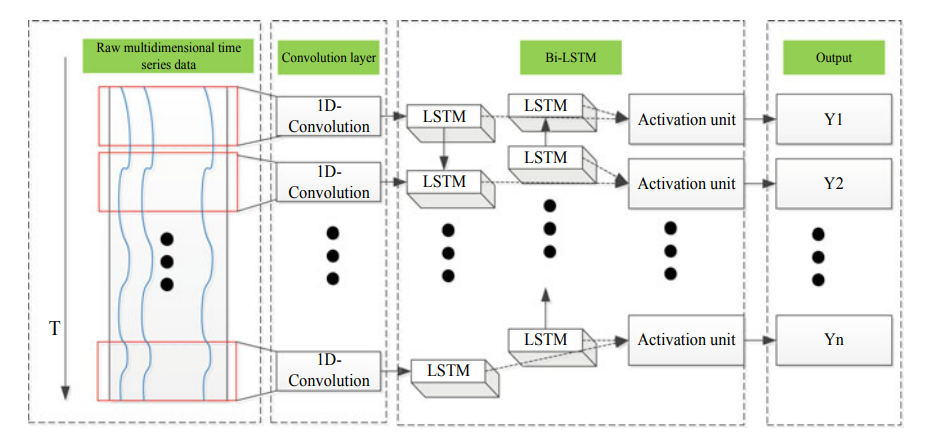
\includegraphics[width = \textwidth]{figures/vfm/lstm_cnn.png}
    \caption{Model framework}
    \label{fig:lstm_cnn}
\end{figure}

Such a network architecture bring together the advantage of time series processing by using LSTM and signal processing for the data that comes from pump sensors by using a 1D convolutional network.

\subsubsection{Convolutional neural networks}
The most recent approach for time series data analysis and important signal processing applications is 1D convolutional neural networks, which can accept data from many input channels. Convolution operation refers to the operation of inner product (multiplication by element and then summation) for different window data and filter matrix (a fixed set of weights). The maxpooling layer is used to reduce the eigenvectors of the convolutional layer output to simplify the computational complexity of the network, at the same time, it performs the feature compression and extracts the main features. The one-dimensional CNN model is shown in fig \ref{fig:cnn_1d}

\begin{figure}
    \centering
    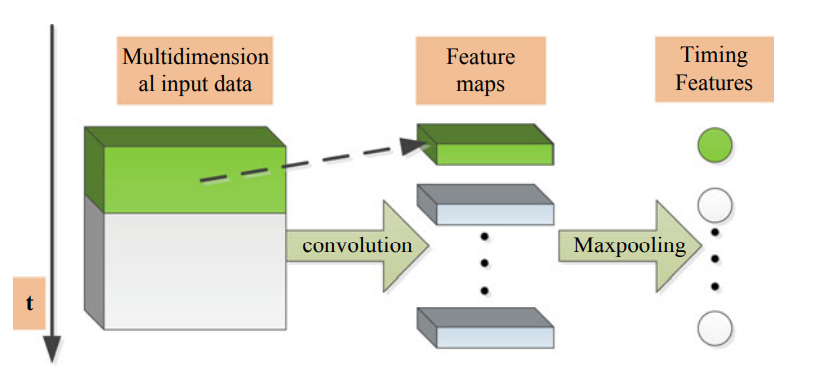
\includegraphics[width = \textwidth]{figures/vfm/cnn_1d.png}
    \caption{One-dimensional convolution}
    \label{fig:cnn_1d}
\end{figure}


\subsubsection{Long short memory algorithm}
\ac{LSTM} is one of the most intricate subfields in deep learning. It is a difficult concept to comprehend. Long Short-Term Memory network adds cells as the information storage module, which
realizes long-term memory of the sequence data, and solves the problem of gradient disappearance and gradient explosion of RNN network.

In the LSTM, the internal states of the unique unit known as the memory cell are used by the architecture to guarantee consistent error flow. Updating the state of the cell through three gating units is the key to LSTM as shown in Fig \ref{fig:lstm_cell}. The three gating units have different calculation methods and function. An input gate, an output gate, and a forget gate make up a typical LSTM unit. 

 \begin{figure}
        \centering
        \resizebox{\columnwidth}{!}{%
        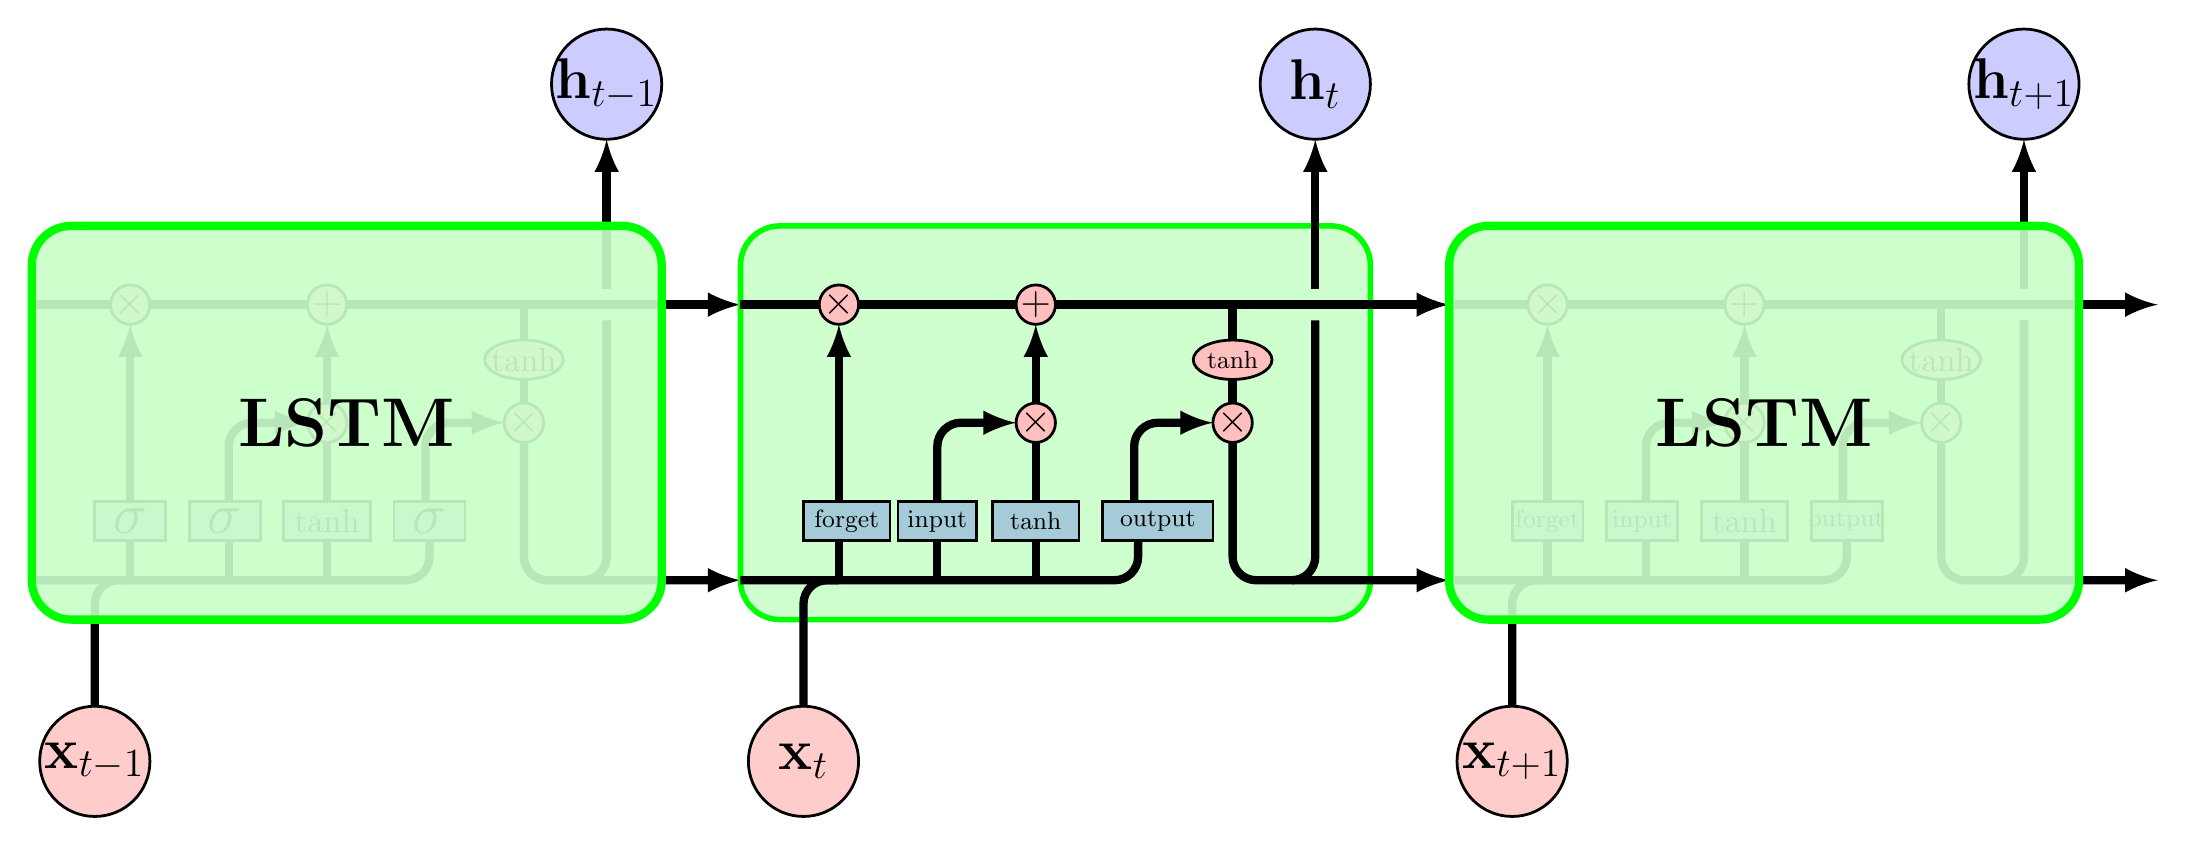
\begin{tikzpicture}
        \coordinate (O) at (0, 0);
        
        \def\offset{0}
        % input
        \filldraw[fill = red,fill opacity=0.2,draw=black,line width=1pt] (-1.2+\offset,0.7) circle (0.7) node[fill opacity=1]{\huge $\mathbf{x}_{t-1}$};
        
        %LSTM
        \filldraw[fill={rgb,255:red,204; green,255; blue,204},fill opacity=0.95,draw=green,line width=2pt,rounded corners=0.5cm] (-2+\offset,2.5) rectangle (6+\offset,7.5); % background
        \filldraw[fill=blue,fill opacity=0.2,draw=black,line width=1pt] (-1.2+\offset,3.5) rectangle (-0.3+\offset,4)node[pos=.5,fill opacity=1]{\huge $\sigma$};
        
        \filldraw[fill=blue,fill opacity=0.2,draw=black,line width=1pt] (0+\offset,3.5) rectangle (0.9+\offset,4)node[pos=.5,fill opacity=1]{\huge $\sigma$};
        
        \filldraw[fill=blue,fill opacity=0.2,draw=black,line width=1pt] (1.2+\offset,3.5) rectangle (2.3+\offset,4)node[pos=.5,fill opacity=1]{\large tanh};
        
        \filldraw[fill=blue,fill opacity=0.2,draw=black,line width=1pt] (2.6+\offset,3.5) rectangle (3.5+\offset,4)node[pos=.5,fill opacity=1]{\huge $\sigma$};
        
        \filldraw[fill=pink,fill opacity=1,draw=black,line width=1pt] (-0.75+\offset,6.5) circle (0.25)node[fill opacity=1]{\Large $\times$};
        
        \filldraw[fill=pink,fill opacity=1,draw=black,line width=1pt] (1.75+\offset,5) circle (0.25)node[fill opacity=1]{\Large $\times$};
        
        \filldraw[fill=pink,fill opacity=1,draw=black,line width=1pt] (4.25+\offset,5) circle (0.25)node[fill opacity=1]{\Large $\times$};
        
        \filldraw[fill=pink,fill opacity=1,draw=black,line width=1pt] (1.75+\offset,6.5) circle (0.25)node[fill opacity=1]{\Large $+$};
        
        \filldraw[fill=pink,fill opacity=1,draw=black,line width=1pt]  (4.25+\offset,5.8) ellipse (0.5cm and 0.25 cm) node[fill opacity=1]{\large tanh};
        
        \draw[ultra thick,black,rounded corners=0.3cm,line width=3pt] (-1.2+\offset,1.4)-- (-1.2+\offset,3)-- (-0.75+\offset,3);
        \draw[ultra thick,black,rounded corners=0.3cm,line width=3pt] (-2+\offset,3)-- (3.05+\offset,3)-- (3.05+\offset,3.5);
        \draw[ultra thick,black,line width=3pt] (-0.75+\offset,3)-- (-0.75+\offset,3.5);
        \draw[-latex,black,line width=3pt] (-0.75+\offset,4)-- (-0.75+\offset,6.25);
        
        \draw[ultra thick,black,line width=3pt] (0.5+\offset,3)-- (0.5+\offset,3.5);
        \draw[-latex,black,rounded corners=0.3cm,line width=3pt] (0.5+\offset,4)-- (0.5+\offset,5)-- (1.5+\offset,5);
        
        \draw[ultra thick,black,line width=3pt] (1.75+\offset,3)-- (1.75+\offset,3.5);
        \draw[ultra thick,black,line width=3pt] (1.75+\offset,4)-- (1.75+\offset,4.75);
        \draw[-latex,black,rounded corners=0.3cm,line width=3pt] (1.75+\offset,5.25)-- (1.75+\offset,6.25);
        
        \draw[ultra thick,black,line width=3pt] (-2+\offset,6.5)-- (-1+\offset,6.5);
        \draw[ultra thick,black,line width=3pt] (-0.5+\offset,6.5)-- (1.5+\offset,6.5);
        \draw[-latex,black,line width=3pt] (2+\offset,6.5)-- (7+\offset,6.5);
        
        \draw[-latex,black,rounded corners=0.3cm,line width=3pt] (3+\offset,4)-- (3+\offset,5)-- (4+\offset,5);
        
        \draw[ultra thick,black,line width=3pt] (4.25+\offset,6.5)-- (4.25+\offset,6.05);
        \draw[ultra thick,black,line width=3pt] (4.25+\offset,5.55)-- (4.25+\offset,5.25);
        \draw[-latex,black,rounded corners=0.3cm,line width=3pt] (4.25+\offset,4.75)-- (4.25+\offset,3)-- (7+\offset,3);
        \draw[ultra thick,black,rounded corners=0.3cm,line width=3pt] (5+\offset,3)-- (5.3+\offset,3) -- (5.3+\offset,6.3);
        \draw[-latex,black,line width=3pt] (5.3+\offset,6.7)-- (5.3+\offset,8.6);
        
        \filldraw[fill = blue,fill opacity=0.2,draw=black,line width=1pt] (5.3+\offset,9.3) circle (0.7)node[fill opacity=1]{\huge $\mathbf{h}_{t-1}$};
        
        \filldraw[fill={rgb,255:red,204; green,255; blue,204},fill opacity=0.9,draw=green,line width=3pt,rounded corners=0.5cm] (-2+\offset,2.5) rectangle (6+\offset,7.5)node[pos=.5,fill opacity=1]{\Huge \textbf{LSTM}};
        
        
        \def\offset{9}
        % input
        \filldraw[fill = red,fill opacity=0.2,draw=black,line width=1pt] (-1.2+\offset,0.7) circle (0.7) node[fill opacity=1]{\huge $\mathbf{x}_{t}$};
        
        %LSTM
        \filldraw[fill={rgb,255:red,204; green,255; blue,204},fill opacity=0.95,draw=green,line width=2pt,rounded corners=0.5cm] (-2+\offset,2.5) rectangle (6+\offset,7.5); % background
        \filldraw[fill=blue,fill opacity=0.2,draw=black,line width=1pt] (-1.2+\offset,3.5) rectangle (-0.1+\offset,4)node[pos=.5,fill opacity=1]{\small forget};
        
        \filldraw[fill=blue,fill opacity=0.2,draw=black,line width=1pt] (0+\offset,3.5) rectangle (1+\offset,4)node[pos=.5,fill opacity=1]{\small input};
        
        \filldraw[fill=blue,fill opacity=0.2,draw=black,line width=1pt] (1.2+\offset,3.5) rectangle (2.3+\offset,4)node[pos=.5,fill opacity=1]{\small tanh};
        
        \filldraw[fill=blue,fill opacity=0.2,draw=black,line width=1pt] (2.6+\offset,3.5) rectangle (4+\offset,4)node[pos=.5,fill opacity=1]{\small output };
        
        \filldraw[fill=pink,fill opacity=1,draw=black,line width=1pt] (-0.75+\offset,6.5) circle (0.25)node[fill opacity=1]{\Large $\times$};
        
        \filldraw[fill=pink,fill opacity=1,draw=black,line width=1pt] (1.75+\offset,5) circle (0.25)node[fill opacity=1]{\Large $\times$};
        
        \filldraw[fill=pink,fill opacity=1,draw=black,line width=1pt] (4.25+\offset,5) circle (0.25)node[fill opacity=1]{\Large $\times$};
        
        \filldraw[fill=pink,fill opacity=1,draw=black,line width=1pt] (1.75+\offset,6.5) circle (0.25)node[fill opacity=1]{\Large $+$};
        
        \filldraw[fill=pink,fill opacity=1,draw=black,line width=1pt]  (4.25+\offset,5.8) ellipse (0.5cm and 0.25 cm) node[fill opacity=1]{\small tanh};
        
        \draw[ultra thick,black,rounded corners=0.3cm,line width=3pt] (-1.2+\offset,1.4)-- (-1.2+\offset,3)-- (-0.75+\offset,3);
        \draw[ultra thick,black,rounded corners=0.3cm,line width=3pt] (-2+\offset,3)-- (3.05+\offset,3)-- (3.05+\offset,3.5);
        \draw[ultra thick,black,line width=3pt] (-0.75+\offset,3)-- (-0.75+\offset,3.5);
        \draw[-latex,black,line width=3pt] (-0.75+\offset,4)-- (-0.75+\offset,6.25);
        
        \draw[ultra thick,black,line width=3pt] (0.5+\offset,3)-- (0.5+\offset,3.5);
        \draw[-latex,black,rounded corners=0.3cm,line width=3pt] (0.5+\offset,4)-- (0.5+\offset,5)-- (1.5+\offset,5);
        
        \draw[ultra thick,black,line width=3pt] (1.75+\offset,3)-- (1.75+\offset,3.5);
        \draw[ultra thick,black,line width=3pt] (1.75+\offset,4)-- (1.75+\offset,4.75);
        \draw[-latex,black,rounded corners=0.3cm,line width=3pt] (1.75+\offset,5.25)-- (1.75+\offset,6.25);
        
        \draw[ultra thick,black,line width=3pt] (-2+\offset,6.5)-- (-1+\offset,6.5);
        \draw[ultra thick,black,line width=3pt] (-0.5+\offset,6.5)-- (1.5+\offset,6.5);
        \draw[-latex,black,line width=3pt] (2+\offset,6.5)-- (7+\offset,6.5);
        
        \draw[-latex,black,rounded corners=0.3cm,line width=3pt] (3+\offset,4)-- (3+\offset,5)-- (4+\offset,5);
        
        \draw[ultra thick,black,line width=3pt] (4.25+\offset,6.5)-- (4.25+\offset,6.05);
        \draw[ultra thick,black,line width=3pt] (4.25+\offset,5.55)-- (4.25+\offset,5.25);
        \draw[-latex,black,rounded corners=0.3cm,line width=3pt] (4.25+\offset,4.75)-- (4.25+\offset,3)-- (7+\offset,3);
        \draw[ultra thick,black,rounded corners=0.3cm,line width=3pt] (5+\offset,3)-- (5.3+\offset,3) -- (5.3+\offset,6.3);
        \draw[-latex,black,line width=3pt] (5.3+\offset,6.7)-- (5.3+\offset,8.6);
        
        \filldraw[fill = blue,fill opacity=0.2,draw=black,line width=1pt] (5.3+\offset,9.3) circle (0.7)node[fill opacity=1]{\huge $\mathbf{h}_{t}$};
        
        %\filldraw[fill={rgb,255:red,204; green,255; blue,204},fill opacity=0.9,draw=green,line width=3pt,rounded corners=0.5cm] (-2+\offset,2.5) rectangle (6+\offset,7.5)node[pos=.5,fill opacity=1]{\Huge \textbf{LSTM}};
        
        
        \def\offset{18}
        % input
        \filldraw[fill = red,fill opacity=0.2,draw=black,line width=1pt] (-1.2+\offset,0.7) circle (0.7) node[fill opacity=1]{\huge $\mathbf{x}_{t+1}$};
        
        %LSTM
        \filldraw[fill={rgb,255:red,204; green,255; blue,204},fill opacity=0.95,draw=green,line width=2pt,rounded corners=0.5cm] (-2+\offset,2.5) rectangle (6+\offset,7.5); % background
        \filldraw[fill=blue,fill opacity=0.2,draw=black,line width=1pt] (-1.2+\offset,3.5) rectangle (-0.3+\offset,4)node[pos=.5,fill opacity=1]{\small forget};
        
        \filldraw[fill=blue,fill opacity=0.2,draw=black,line width=1pt] (0+\offset,3.5) rectangle (0.9+\offset,4)node[pos=.5,fill opacity=1]{\small input};
        
        \filldraw[fill=blue,fill opacity=0.2,draw=black,line width=1pt] (1.2+\offset,3.5) rectangle (2.3+\offset,4)node[pos=.5,fill opacity=1]{\large tanh};
        
        \filldraw[fill=blue,fill opacity=0.2,draw=black,line width=1pt] (2.6+\offset,3.5) rectangle (3.5+\offset,4)node[pos=.5,fill opacity=1]{\small output};
        
        \filldraw[fill=pink,fill opacity=1,draw=black,line width=1pt] (-0.75+\offset,6.5) circle (0.25)node[fill opacity=1]{\Large $\times$};
        
        \filldraw[fill=pink,fill opacity=1,draw=black,line width=1pt] (1.75+\offset,5) circle (0.25)node[fill opacity=1]{\Large $\times$};
        
        \filldraw[fill=pink,fill opacity=1,draw=black,line width=1pt] (4.25+\offset,5) circle (0.25)node[fill opacity=1]{\Large $\times$};
        
        \filldraw[fill=pink,fill opacity=1,draw=black,line width=1pt] (1.75+\offset,6.5) circle (0.25)node[fill opacity=1]{\Large $+$};
        
        \filldraw[fill=pink,fill opacity=1,draw=black,line width=1pt]  (4.25+\offset,5.8) ellipse (0.5cm and 0.25 cm) node[fill opacity=1]{\large tanh};
        
        \draw[ultra thick,black,rounded corners=0.3cm,line width=3pt] (-1.2+\offset,1.4)-- (-1.2+\offset,3)-- (-0.75+\offset,3);
        \draw[ultra thick,black,rounded corners=0.3cm,line width=3pt] (-2+\offset,3)-- (3.05+\offset,3)-- (3.05+\offset,3.5);
        \draw[ultra thick,black,line width=3pt] (-0.75+\offset,3)-- (-0.75+\offset,3.5);
        \draw[-latex,black,line width=3pt] (-0.75+\offset,4)-- (-0.75+\offset,6.25);
        
        \draw[ultra thick,black,line width=3pt] (0.5+\offset,3)-- (0.5+\offset,3.5);
        \draw[-latex,black,rounded corners=0.3cm,line width=3pt] (0.5+\offset,4)-- (0.5+\offset,5)-- (1.5+\offset,5);
        
        \draw[ultra thick,black,line width=3pt] (1.75+\offset,3)-- (1.75+\offset,3.5);
        \draw[ultra thick,black,line width=3pt] (1.75+\offset,4)-- (1.75+\offset,4.75);
        \draw[-latex,black,rounded corners=0.3cm,line width=3pt] (1.75+\offset,5.25)-- (1.75+\offset,6.25);
        
        \draw[ultra thick,black,line width=3pt] (-2+\offset,6.5)-- (-1+\offset,6.5);
        \draw[ultra thick,black,line width=3pt] (-0.5+\offset,6.5)-- (1.5+\offset,6.5);
        \draw[-latex,black,line width=3pt] (2+\offset,6.5)-- (7+\offset,6.5);
        
        \draw[-latex,black,rounded corners=0.3cm,line width=3pt] (3+\offset,4)-- (3+\offset,5)-- (4+\offset,5);
        
        \draw[ultra thick,black,line width=3pt] (4.25+\offset,6.5)-- (4.25+\offset,6.05);
        \draw[ultra thick,black,line width=3pt] (4.25+\offset,5.55)-- (4.25+\offset,5.25);
        \draw[-latex,black,rounded corners=0.3cm,line width=3pt] (4.25+\offset,4.75)-- (4.25+\offset,3)-- (7+\offset,3);
        \draw[ultra thick,black,rounded corners=0.3cm,line width=3pt] (5+\offset,3)-- (5.3+\offset,3) -- (5.3+\offset,6.3);
        \draw[-latex,black,line width=3pt] (5.3+\offset,6.7)-- (5.3+\offset,8.6);
        
        \filldraw[fill = blue,fill opacity=0.2,draw=black,line width=1pt] (5.3+\offset,9.3) circle (0.7)node[fill opacity=1]{\huge $\mathbf{h}_{t+1}$};
        
        \filldraw[fill={rgb,255:red,204; green,255; blue,204},fill opacity=0.9,draw=green,line width=3pt,rounded corners=0.5cm] (-2+\offset,2.5) rectangle (6+\offset,7.5)node[pos=.5,fill opacity=1]{\Huge \textbf{LSTM}};
        \end{tikzpicture}
         }
\caption{Structure of LSTM cells}
\label{fig:lstm_cell}
\end{figure}

Forget Gate: The sigmoid function generates a value between 0 and 1 in the forget gate, which is the first step, to indicate how much knowledge of the prior hidden state and the present input it should keep. Input Gate:The following action has two components. The input gate chooses the new data to be stored in the memory cell first. A tanh layer then creates a vector of new candidate values that will be added to the state. Output gate : Applying the sigmoid function to the prior hidden state and current input and multiplying it by the tanh function applied to the new memory cell will provide values between -1 and 1 for the memory cell's output. The equations for the forget, input and output gates in LSTM are presented in \ref{Eq:forget_lstm}, \ref{Eq:output_lstm}:

\begin{equation}\label{Eq:forget_lstm}
    f_t\ =\sigma (w_f[h^{t-1},x^t]+b_f)
\end{equation}

\begin{equation}\label{Eq:input_lstm}
    i_t\ =\ \sigma\ (w_i[h^{t-1},x^t]+b_i)
\end{equation}

\begin{equation}\label{Eq:output_lstm}
    o_t\ =\sigma (w_o[h^{t-1},x^t]+b_o)
\end{equation}

Where :
$I_t$ = represents the input gate.\\
$F_t$ = represents the forget gate.\\
$O_t$ = represents the output gate. \\
$\sigma$ = represents sigmoid function.\\
$W_x$= weight for the respective gate (x) neurons.\\
$H^{t-1}$ = output of the previous lstm block (at timestamp t-1)\\
$X^t$ =input at current timestamp. \\
%$B_x$ = biases for the respective gates (X)
	
The equations for the cell state, candidate cell state and the final output:
\begin{equation}
   \tilde{C}^t = tanh (wc [ht-1,xt]+ bc ) 
\end{equation}

\begin{equation}
    C^t\ =\ F_t\ \times C^{t-1}+I_t\times \tilde{C}^t
\end{equation}

\begin{equation}
    H_t\ =\ o_t\times tanh(C^t)
\end{equation}
Where :
$Ct$ = cell state (memory) at timestamp (t).\\
$\tilde{C}^t$ = represents candidate for cell state at timestamp (t).\\

The gate units of the bidirectional LSTM are identical to the LSTM. Bi-LSTM is a combination of a forward LSTM and a backward LSTM, that means, one time step of data is input simultaneously in both forward and reverse directions. Although Bi-LSTM needs to train more generations to converge to stability, it also has higher precision because it gets more input information. So we chose the Bi-LSTM as the prediction model.

\section{Experiments}
% symbolic regression generations and population

%neural networks and hyperparamters tuning 
In this section, we will validate and evaluate the proposed models using the electrical submersible pumps data set that we have explored earlier this chapter. 


When we usually use neural networks to build models, the size of the network layer
and the number of neurons are not strictly defined. We determined the parameters of each layer of the model through multiple experimental adjustments. Specifically, we set up two layers of convolution layers, the filters size of each convolution layer was set to 3, and the Relu function was used. Two layers of Bi-LSTM, the previous layer of neurons was set to 30, and the latter layer was set to 24 which is determined by the output dimension of the model. In addition, all models are supervised trained using Adam algorithm that optimizes a predetermined objective function, to obtain model

\section{Summary}
In order to monitor and improve the production processes, it is crucial to estimate multiphase flowrates correctly. In typical field operations, the estimation of well flowrates is done by directing stream from a specific well into a test separator where it is split into oil, gas and water. This traditional method has a disadvantage of not being able to identify production trends. Another technology is invented to estimate production rates by measuring one physical property of the stream and relate it to different fluids rates. It is called multiphase flow metes (MPFMs). The aforementioned methods have high capital and operating expenses for such meter’s maintenance. 

A solution involving machine learning and physics based transient modeling is an alternative to the usage of MPFMs and production testing. It is called virtual flow meters (VFM). It arises as an attractive research area in oil and gas industry. It depends on either analytical or data driven models for real time calculations of production phases.

In this chapter, a new data driven model was introduced to calculate the multiphase flow rate using sensors measurements of the electrical submersible pumps. In addition, a framework is introduced for detailed exploratory data analysis and calibrating the proposed model to account for production conditions. Then, feature prioritization experiments are conducted to identify the most dominant parameters that affects rates prediction. Finally, the mean absolute error, mean squared error, and r squared are used to compare the models. 

In this work we have used a real time data set from ESP assisted wells. Our method encompassed the implementation of symbolic regression, and deep learning. Convolutional neural network pipeline with long short term memory algorithm (LSTM) are used for real time prediction of liquid rate and water cut based on sensors’ data.  


